%% ---------------------------------------------------------------------
%% Copyright 2014, Thales, IGN, Rémi Cura
%% 
%% This file contains the introduction of article
%% ---------------------------------------------------------------------


\section{Introduction}

\begin{figure*}[t!]
	\begin{center}
		\fbox{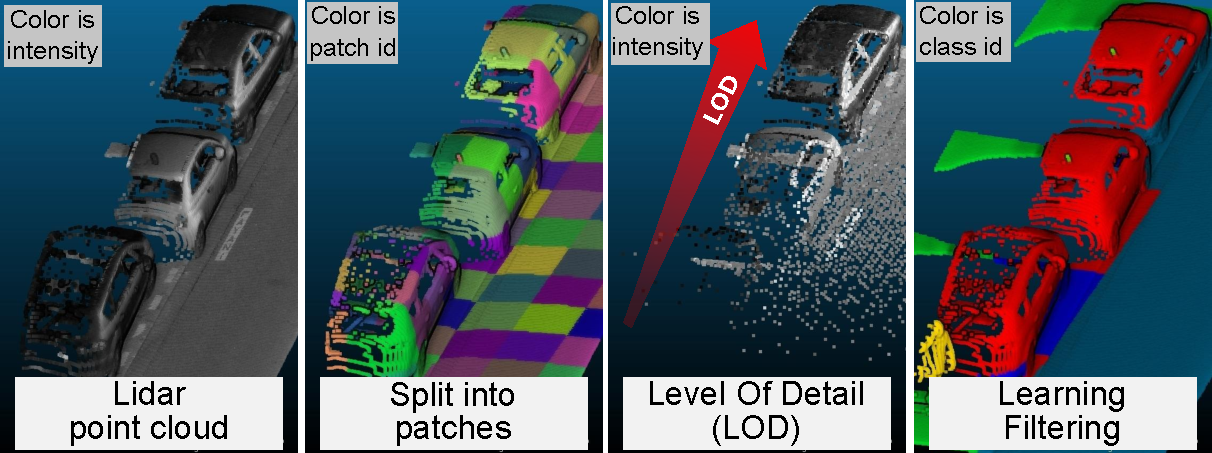
\includegraphics[width=\textwidth,keepaspectratio ]{./illustrations/chap2/lod_banner/banner_for_paper}}
		\caption{Graphical Abstract : a Lidar point cloud (1), is split it into patches (2) 
		and stored in the PCS (\cite{Cura2015}), patches are re-ordered to obtain free LOD 
		(3) (a gradient of LOD here), lastly the ordering by-product is a multiscale dimensionality descriptor used as a feature for learning and efficient filtering (4).} 
		\label{lod.fig:banner_image}
	\end{center}
\end{figure*} 

\subsection{Problem}  
	Point cloud data is becoming more and more common. Following the same trend, the acquisition frequency and precision of the Lidar device are also increasing.
	Thus point cloud processing is entering in the Big Data realm.
	Point cloud data usage is also spreading and going out of their traditional user communities. 
	Lidar data are now commonly used by non-specialized users. 
	The now common datasets in the multi billion point range can not fit in computer memory. 
	Furthermore, having the complete and fully detailed point cloud is impracticable, unnecessary, or even damageable for most applications.
	
	The ability to reduce the number of points is then vital for practical point cloud management and usage.
 
	\myimage{"./illustrations/chap2/two_reduction_strategy/two_reduction_strategy"}{Two strategies to limit the amount of points to work on.}{lod.fig:two_reduction} 
	
	There are basically two levers to reduce the amount of data considered (See Figure \ref{lod.fig:two_reduction}). The first would be \textbf{filtering} data based on its characteristics (position, time, semantic, etc.), thus keeping the original data, but only a portion of it.
	The second lever would be to \textbf{generalise} the data, that is replace many points with few objects that represent  well those points. Those objects can be more abstract (geometric primitives like plane for example), or of the same type, i.e. simply some well chosen points (subset).
	
	For instance, to visualize a part of a massive point cloud, we might fetch only the points that are visible (filtering),
	and not display the totality of selected points, but only points better representing the scene (generalisation).
	
	The Point Cloud Server (PCS) we propose un \cite{cura2015} is compatible with filtering and generalization. It extensively covers the filtering part, with many possibilities (spatial, semantic, attributes, using vector and raster data, using metadata). The PCS also use generalisation of points in the form of more abstract types (bounding box, planes, stats, etc.).
	In this article, we explore the last option: how to generalise groups of points by choosing a representative subset of points (See Fig. \ref{lod.fig:two_reduction}).
	
	This kind of problem is common in Geographical Information System (GIS): how to generalize information contained in huge datasets, that is reduce the details of data while retaining its principal organisation.
	
	This problem is also much broader and very commons across research field. It could be seen as compression, clustering, dimensionality reduction, or Level Of Detail (LOD) if the goal is visualisation.
	
	In this article, we consider successive reducion of the amount of points in several levels while preserving the geometric characteristics of the underlying sensed object, in an efficient manner, and while being robust point density variation. The goal is not only visualization of large point cloud, but mainly processing of large point clouds.
	
	Robustness to variation of density is necessary because the sensing may be structured for the sensing device (for instance a Lidar may sense point using a constant angle), but not necessary for the sensed object (see Fig. \ref{lod.fig:irregular_sampling}). Furthermore,fusing multiple point clouds also produce non regular density.
	\myimage{"./illustrations/chap2/problem_in_sampling/regular_vs_irregular_sampling"}{Regular sensing does not imply regular sampling.}{lod.fig:irregular_sampling}.
	

\subsection{Related Work} 

	Sophisticated methods have been proposed to generalise 2D points for cartographic applications. \cite{Sester2001} uses Self Organizing Maps, \cite{Schwartges2013} uses Active Range and (mixed) integer
	linear programming.
	In both case, the goal is a very specific type of visualisation (cartography), and it obviously relies on having a 2D plan on which perform the methods.
	Applying directly such methods to point clouds would thus require to have access to surfaces of sensed objects.
	
	Yet, getting this surface (reconstruction) is a very hard challenge, sometime not even possible, and thus we can not rely on it.
	
	Because the goal si to produce hierarchical levels of points, it seems natural to use a hierarchical structure to compute those levels.
	\cite{Rusinkiewicz2000} use a Bounding Sphere Hierarchy for a visualisation application.
	On the other hand, Octree (\cite{Meagher1982}) have become the de-facto choice.
	Indeed, they can be build efficiently ordering points by Morton order (\cite{Feng2014}),
	which is similar in principle to GeoHash (\cite{Sabo2014}).
	Octree can even be created out of memory for extremely large point clouds (\cite{Baert2014}). 
	
	Moreover, their regularity allows efficient representation and compression (\cite{Schnabel2006,Huang2006}), as well as fast geospatial access to data (\cite{Elseberg2013}).
	Octree are also natural condidates to nesting (i.e. create a hierarchy of octrees with various resolution and occupancy, as in \cite{Hornung2013}). 
	
	
	\cite{Bereuter2015} recently gave an overview of how quad tree can be used for point generalisation.
	The steps are first to compute a tree for the point cloud.
	Then, the point generalisation at a given level is obtained for each cell of the same tree level, by having one point represent all the points of this cell.
	
	There are two methods to choose a point representing the others. The first one is to select on points among all ('select').
	The second method is to create a new point that will represent well the others ('aggregate'). 
	Both these methods can use geometry of points, but also other attributes.
	
	In theory, choosing an optimal point would also depend on application.
	For instance lets consider a point cloud containing a classification, and suppose the application is to visually identify the presence of a very rarely present class C.
	In this case a purely geometrical LOD would probably hide C until the very detailed levels. On the opposite, prefering a point classified in C whenever possible would be optimal for this application.
	
	However, a LOD method has to be agnostic regarding point clouds,
	and point clouds may have many attributes of various type and meaning, as long as many applications.
	Therefore, most methods use only the minimal common factor of possible attributes, that is spatial coordinates. 
	For visualisation applications, aggregating points seems to be the most popular choice \cite{Schutz2015,Hornung2013,Elseberg2013}. with aggregating functions like centroids of the points or centroid of the cell.
	
	All of this methods also use an aggregative function (barycentre of the points, centroid of the cell) to represent the points of a cell.
	Using the barycentre seems intuitive, as it is also the point that minimize the squared distance to other points in the cell, and thus a measure of geometric error.
	
	However, using the 'aggregate' rather than 'select' strategy necessary introduces aggregating errors
	 (as opposed to potential aliasing error), and is less agnostic.
	Indeed, aggregating means fabricating new points, and also necessitate a way to aggregate for each attributes, which might be complex (for instance semantic aggregating; a point of trash can and a point of bollard could be aggregated into a point of street furniture).
	This might not be a problem for visualization application.
	Yet our goal is to provide LOD for other processing methods, which might be influenced by aggregating errors.
	Furthermore, the barycentre is very sensible to density variations.
	
	Therefore, we prefer to use a 'select' strategy. The point to be selected is the closest to the centroid of the octree cell.
	If the point cloud density is sufficient this strategy produces a nearly regularly sampled point cloud, which might be a statistical advantage for processing methods. 
	To establish a parallel with statistics, picking one point per cell is akin to a Latin Hypercube (see \cite{McKay1979}).
	Avoiding the averaging strategy might also increase the quantity of information than can be retrieved (similar to compressed sensing, see \cite{Fornasier2010}).
	
	
	We note that most of the LOD systems seems to have been created to first provide a fast access to point (spatial indexing), and then adapted to provide LOD.
	Using the PCS, we can separate the indexing part, and the LOD scheme. From this stems less design constraints, more possibilities, and a method than is not dedicated to only one application (like visualisation). 
	

\subsection{Contribution}

	This paper re-uses and combines existing and well established methods with a focus on simplicity and efficiency. As such, all the methods are tested on billions scale point cloud, and are Open Source for sake of reproducibility test and improvements.
	
	Our first contribution is to store the LOD implicitly in the ordering of the points rather than externally, avoiding any data duplication.
	Thus, we don't duplicate information, and the more we read points, the more precise of an approximation of the point cloud we get. If we read all the points, we have the original point cloud.
	
	The second contribution (MidOc) is a simple way to order points in order to have an increasingly better geometric approximation of the point cloud when following this order.
	
	The third contribution is to show that this ordering embed information about the dimensionality of the sensed object,
	to the point of being a simple multi-scale dimensionality descriptor.
	We demonstrate the interest of this descriptor by comparing it to a state of the art dimensionality descriptor, then by assessing it potential by performing a Random Forest classification that can then be used for very fast pre-filtering of points, and other applications.
		
	
\subsection{Plan of the article}
	The rest of this article is organized as follows:
	in the next section \ref{lod.sec:method} we present the methods.  
	In the result section \ref{lod.sec:result} we give the results.
	We discuss it and the possible limitations in section \ref{lod.sec:discussion}.
	
	Following the IMRAD format~\citep{Wu2011}, the remainder of this article is divided into three sections.
	Section~\ref{lod.sec:method} presents the LOD solution, how it produces a dimensionality descriptor, and how this can leveraged for classification.  
	Section~\ref{lod.sec:result} reports on the experiments validating the methods.
	Finally, the details, the limitations, and potential applications are discussed in Section~\ref{lod.sec:discussion}.
	
